\documentclass[aspectratio=169, 12pt]{beamer}

% ── Theme ──
\usetheme{Madrid}
\usecolortheme{default}
\setbeamertemplate{navigation symbols}{}
\setbeamertemplate{footline}[frame number]
\setbeamertemplate{itemize items}[circle]
\setbeamertemplate{enumerate items}[default]

% ── Packages ──
\usepackage[utf8]{inputenc}
\usepackage[T1]{fontenc}
\usepackage{booktabs}
\usepackage{tikz}
\usetikzlibrary{shapes.geometric, arrows.meta, positioning, calc}
\usepackage{pgfplots}
\pgfplotsset{compat=1.18}
\usepackage{tabularx}

% ── Colours ──
\definecolor{irpgblue}{HTML}{2563EB}
\definecolor{vicamber}{HTML}{D97706}
\definecolor{goldgreen}{HTML}{059669}
\definecolor{accent}{HTML}{6366F1}

\setbeamercolor{frametitle}{fg=white, bg=irpgblue}
\setbeamercolor{title}{fg=white, bg=irpgblue}
\setbeamercolor{structure}{fg=irpgblue}
\setbeamercolor{block title}{bg=irpgblue!15, fg=irpgblue}
\setbeamercolor{block body}{bg=irpgblue!5}

% ══════════════════════════════════════════════════════════════
\title{Weekly Progress Update}
\subtitle{Pipeline Improvements, External Benchmarks \& Neo4j}
\author{Safaa Salman}
\date{\today}

\begin{document}

% ──────────────────────────────────────────────────────────────
\begin{frame}
\titlepage
\end{frame}

% ──────────────────────────────────────────────────────────────
\begin{frame}{This Week's Agenda}
\begin{enumerate}
    \item \textbf{Phase 1}: Fix edge extraction (prompt + review + few-shot)
    \item \textbf{Phase 2}: Upgrade PDF parsing (Docling for tables)
    \item \textbf{Phase 3}: Expand evaluation framework
    \item \textbf{External benchmarks}: PET + BREX
    \item \textbf{Neo4j}: Graph database deployment
    \item \textbf{Results \& next steps}
\end{enumerate}
\end{frame}

% ══════════════════════════════════════════════════════════════
\section{Phase 1: Fix Edge Extraction}
% ══════════════════════════════════════════════════════════════

% ──────────────────────────────────────────────────────────────
\begin{frame}{The Problem: Edge F1 = 0.414}
\begin{columns}
\begin{column}{0.55\textwidth}
\textbf{Three root causes:}
\begin{itemize}
    \item Decision branches merged into linear paths
    \item Condition labels vague (``Yes''/``No'')
    \item Over-extraction: invented sub-steps
\end{itemize}
\end{column}
\begin{column}{0.42\textwidth}
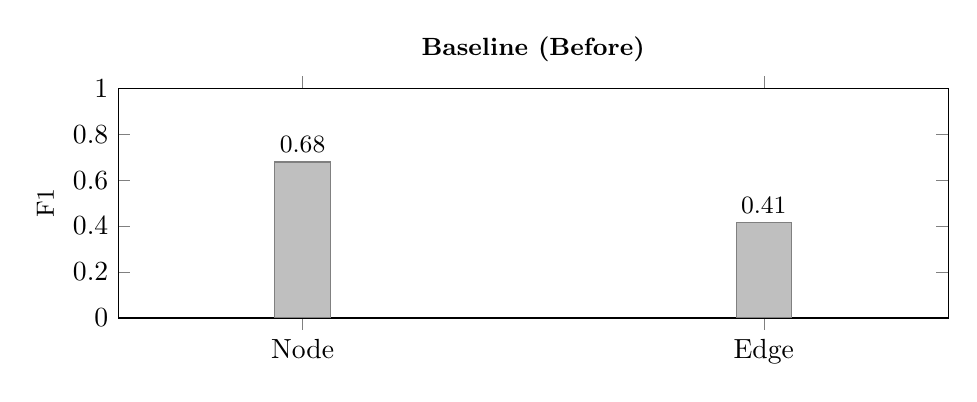
\begin{tikzpicture}
\begin{axis}[
    ybar, bar width=20pt,
    width=\textwidth, height=4.5cm,
    ylabel={F1}, ylabel style={font=\small},
    symbolic x coords={Node, Edge},
    xtick=data, ymin=0, ymax=1,
    nodes near coords, every node near coord/.style={font=\small\bfseries},
    enlarge x limits=0.4,
    title={\small Baseline (Before)},
    title style={font=\small\bfseries},
]
\addplot[fill=gray!50, draw=gray] coordinates {(Node, 0.679) (Edge, 0.414)};
\end{axis}
\end{tikzpicture}
\end{column}
\end{columns}
\end{frame}

% ──────────────────────────────────────────────────────────────
\begin{frame}{Solution: Four Changes}
\begin{enumerate}
    \item \textbf{21-rule SYSTEM\_PROMPT}
    \begin{itemize}
        \item Rules 8--14: explicit edge \& branching patterns
        \item Rules 15--18: anti-over-extraction
    \end{itemize}
    \item \textbf{Triage as 3rd few-shot example}
    \begin{itemize}
        \item 15 nodes, 20 edges, 5 decision nodes
        \item Teaches complex branching by example
    \end{itemize}
    \item \textbf{Edge review pass} (GPT-4o-mini)
    \begin{itemize}
        \item 6 checks on edge completeness
        \item Safeguard: only accept if issues decrease
    \end{itemize}
    \item \textbf{TextFlow} for diagram protocols
    \begin{itemize}
        \item Image $\rightarrow$ Mermaid $\rightarrow$ protocol graph
    \end{itemize}
\end{enumerate}
\end{frame}

% ──────────────────────────────────────────────────────────────
\begin{frame}{Phase 1 Results: Edge F1 Nearly Doubled}
\centering
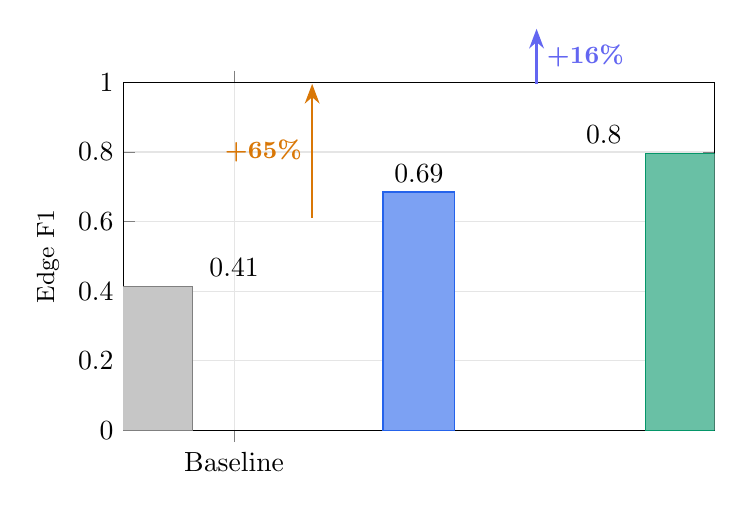
\begin{tikzpicture}
\begin{axis}[
    ybar, bar width=26pt,
    width=0.75\textwidth, height=6cm,
    ylabel={Edge F1}, ylabel style={font=\small},
    symbolic x coords={Baseline, Round 1, Round 2},
    xtick=data, ymin=0, ymax=1.0,
    nodes near coords, every node near coord/.style={font=\normalsize\bfseries},
    enlarge x limits=0.3,
    grid=major, grid style={gray!20},
]
\addplot[fill=gray!45, draw=gray] coordinates {(Baseline, 0.414)};
\addplot[fill=irpgblue!60, draw=irpgblue] coordinates {(Round 1, 0.685)};
\addplot[fill=goldgreen!60, draw=goldgreen] coordinates {(Round 2, 0.795)};
\end{axis}
\draw[-{Stealth[length=2.5mm]}, thick, vicamber] (2.4,2.7) -- (2.4,4.4) node[midway, left, font=\small\bfseries, text=vicamber] {+65\%};
\draw[-{Stealth[length=2.5mm]}, thick, accent] (5.25,4.4) -- (5.25,5.1) node[midway, right, font=\small\bfseries, text=accent] {+16\%};
\end{tikzpicture}

\vspace{0.3cm}
\footnotesize Round 1 = prompt + edge review + Triage few-shot \quad|\quad Round 2 = + anti-over-extraction rules
\end{frame}

% ══════════════════════════════════════════════════════════════
\section{Phase 2 \& 3}
% ══════════════════════════════════════════════════════════════

% ──────────────────────────────────────────────────────────────
\begin{frame}{Phase 2: Docling for Table Parsing}
\begin{columns}
\begin{column}{0.5\textwidth}
\textbf{Problem:} $\sim$15 table-format sections \\[0.3em]
PyMuPDF loses row/column structure

\vspace{0.5cm}
\textbf{Solution:}
\begin{itemize}
    \item IBM Docling (DocLayNet + TableFormer)
    \item Routes only \texttt{table} sections through Docling
    \item PyMuPDF remains default (faster)
    \item Dedicated \texttt{TABLE\_EXTRACTION\_PROMPT}
\end{itemize}
\end{column}
\begin{column}{0.47\textwidth}
\begin{block}{Routing Logic}
\small
\texttt{if format == "table":}\\
\quad \texttt{text = docling(pdf)}\\
\texttt{else:}\\
\quad \texttt{text = pymupdf(pdf)}
\end{block}
\vspace{0.3cm}
\begin{block}{Table Prompt}
\small
Row $\rightarrow$ condition-action pair\\
Condition col $\rightarrow$ decision node\\
Action col $\rightarrow$ action node
\end{block}
\end{column}
\end{columns}
\end{frame}

% ──────────────────────────────────────────────────────────────
\begin{frame}{Phase 3: Evaluation Expansion}
\textbf{New metrics added to \texttt{evaluate.py}:}
\vspace{0.3cm}
\begin{itemize}
    \item \textbf{Edge Condition Similarity} --- text similarity of condition labels
    \item \textbf{Condition Exact Match Rate} --- \% matching at $\geq$0.8
    \item \textbf{Branching Accuracy} --- \% of decision nodes with correct outgoing edge count
    \item \textbf{Path Count} --- distinct start$\rightarrow$end paths (DFS, depth limit 50)
\end{itemize}

\vspace{0.5cm}
\begin{center}
\begin{tabular}{lcc}
\toprule
\textbf{Metric} & \textbf{Baseline} & \textbf{After Phase 1--3} \\
\midrule
Condition Similarity & 0.746 & \textbf{0.889} (+19\%)\\
Branching Accuracy   & 0.944 & \textbf{1.000} \\
\bottomrule
\end{tabular}
\end{center}
\end{frame}

% ══════════════════════════════════════════════════════════════
\section{Updated Pipeline}
% ══════════════════════════════════════════════════════════════

% ──────────────────────────────────────────────────────────────
\begin{frame}{Updated Pipeline: 6 $\rightarrow$ 7 Stages}
\centering
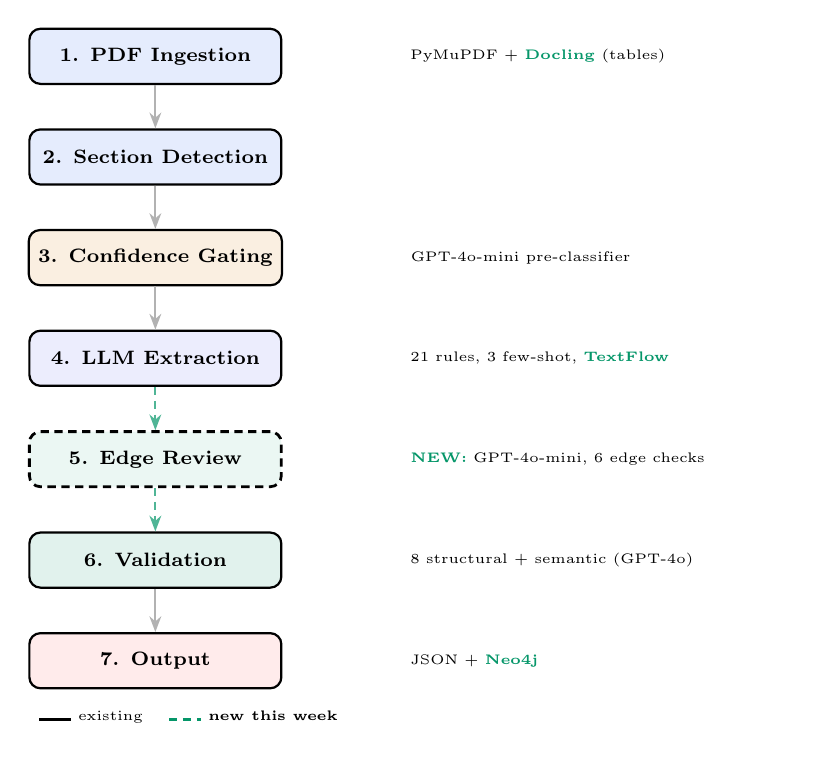
\begin{tikzpicture}[
    node distance=0.55cm,
    stg/.style={draw, rounded corners=4pt, minimum width=3.2cm, minimum height=0.7cm, align=center, font=\scriptsize\bfseries, thick},
    newstg/.style={draw, rounded corners=4pt, minimum width=3.2cm, minimum height=0.7cm, align=center, font=\scriptsize\bfseries, thick, densely dashed, line width=1pt},
    det/.style={font=\tiny, align=left, text width=4.8cm},
    arr/.style={-{Stealth[length=2mm]}, thick, gray!60},
    newarr/.style={-{Stealth[length=2mm]}, thick, goldgreen!70, densely dashed},
]
    \node[stg, fill=irpgblue!12] (s1) {1. PDF Ingestion};
    \node[stg, fill=irpgblue!12, below=of s1] (s2) {2. Section Detection};
    \node[stg, fill=vicamber!12, below=of s2] (s3) {3. Confidence Gating};
    \node[stg, fill=accent!12, below=of s3] (s4) {4. LLM Extraction};
    \node[newstg, fill=goldgreen!8, below=of s4] (s5) {5. Edge Review};
    \node[stg, fill=goldgreen!12, below=of s5] (s6) {6. Validation};
    \node[stg, fill=red!8, below=of s6] (s7) {7. Output};

    \draw[arr] (s1) -- (s2);
    \draw[arr] (s2) -- (s3);
    \draw[arr] (s3) -- (s4);
    \draw[newarr] (s4) -- (s5);
    \draw[newarr] (s5) -- (s6);
    \draw[arr] (s6) -- (s7);

    % Details (right side)
    \node[det, right=1.5cm of s1] {PyMuPDF + \textcolor{goldgreen}{\textbf{Docling}} (tables)};
    \node[det, right=1.5cm of s3] {GPT-4o-mini pre-classifier};
    \node[det, right=1.5cm of s4] {21 rules, 3 few-shot, \textcolor{goldgreen}{\textbf{TextFlow}}};
    \node[det, right=1.5cm of s5] {\textcolor{goldgreen}{\textbf{NEW:}} GPT-4o-mini, 6 edge checks};
    \node[det, right=1.5cm of s6] {8 structural + semantic (GPT-4o)};
    \node[det, right=1.5cm of s7] {JSON + \textcolor{goldgreen}{\textbf{Neo4j}}};

    % Legend
    \node[font=\tiny, anchor=north west] at ([yshift=-0.15cm]s7.south west) {
        \tikz{\draw[thick] (0,0) -- (0.4,0);} existing \quad
        \tikz{\draw[thick, densely dashed, goldgreen] (0,0) -- (0.4,0);} \textbf{new this week}
    };
\end{tikzpicture}
\end{frame}

% ══════════════════════════════════════════════════════════════
\section{Phase 1--3 Summary}
% ══════════════════════════════════════════════════════════════

% ──────────────────────────────────────────────────────────────
\begin{frame}{Phase 1--3: All Metrics}
\centering
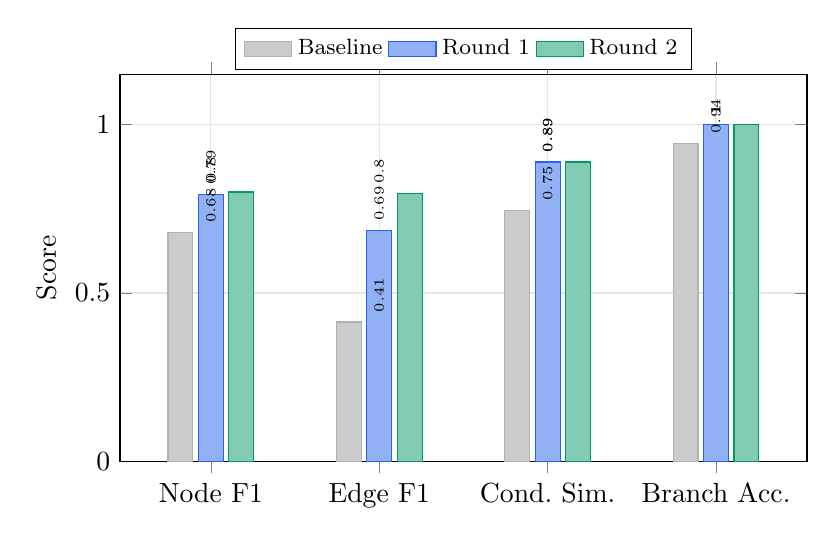
\begin{tikzpicture}
\begin{axis}[
    ybar, bar width=9pt,
    width=0.85\textwidth, height=6.5cm,
    ylabel={Score},
    symbolic x coords={Node F1, Edge F1, Cond.\ Sim., Branch Acc.},
    xtick=data, ymin=0, ymax=1.15,
    legend style={at={(0.5,1.12)}, anchor=north, legend columns=3, font=\footnotesize},
    nodes near coords, every node near coord/.style={font=\tiny, rotate=90, anchor=west},
    enlarge x limits=0.18,
    grid=major, grid style={gray!20},
    area legend,
]
\addplot[fill=gray!40, draw=gray!60] coordinates {
    (Node F1, 0.679) (Edge F1, 0.414) (Cond.\ Sim., 0.746) (Branch Acc., 0.944)
};
\addplot[fill=irpgblue!50, draw=irpgblue] coordinates {
    (Node F1, 0.792) (Edge F1, 0.685) (Cond.\ Sim., 0.889) (Branch Acc., 1.000)
};
\addplot[fill=goldgreen!50, draw=goldgreen] coordinates {
    (Node F1, 0.800) (Edge F1, 0.795) (Cond.\ Sim., 0.889) (Branch Acc., 1.000)
};
\legend{Baseline, Round 1, Round 2}
\end{axis}
\end{tikzpicture}

\vspace{0.2cm}
\small Edge F1: \textbf{+92\%} \quad Node F1: \textbf{+18\%} \quad Condition Sim: \textbf{+19\%} \quad Branching: \textbf{100\%}
\end{frame}

% ══════════════════════════════════════════════════════════════
\section{External Benchmarks}
% ══════════════════════════════════════════════════════════════

% ──────────────────────────────────────────────────────────────
\begin{frame}{Why External Benchmarks?}
\begin{itemize}
    \item Our gold standards: \textbf{5 protocols, 1 annotator}
    \item Need to validate generalisation beyond IRPG
    \item Two independent benchmarks selected:
\end{itemize}

\vspace{0.4cm}
\begin{columns}
\begin{column}{0.48\textwidth}
\begin{block}{PET (Neuberger 2024)}
\small
\begin{itemize}
    \item 45 English process descriptions
    \item BPMN annotations (activities, gateways, flows)
    \item GPT-4o baseline: Activity F1 = 0.740
\end{itemize}
\end{block}
\end{column}
\begin{column}{0.48\textwidth}
\begin{block}{BREX (Yang 2025)}
\small
\begin{itemize}
    \item 409 Chinese business regulations
    \item 2,855 condition-action rules
    \item \textbf{Cross-lingual test} (English prompts)
\end{itemize}
\end{block}
\end{column}
\end{columns}
\end{frame}

% ──────────────────────────────────────────────────────────────
\begin{frame}{Challenge: Annotation Granularity Mismatch (PET)}
\begin{center}
\begin{tabular}{lll}
\toprule
& \textbf{PET Gold} & \textbf{Our Extraction} \\
\midrule
Activity & ``brings in'' & ``The customer brings in the defective...'' \\
Gateway  & ``If'' & ``Is the defect covered under warranty?'' \\
Activity & ``checks'' & ``The technician checks the hardware...'' \\
\bottomrule
\end{tabular}
\end{center}

\vspace{0.5cm}
\textbf{Solution: Token-overlap similarity}
\begin{itemize}
    \item Fuzzy match each gold token against extracted tokens
    \item Recall-dominated scoring for 1--2 word gold spans
    \item Threshold = 0.3 (vs.\ standard 0.5)
\end{itemize}
\end{frame}

% ──────────────────────────────────────────────────────────────
\begin{frame}{PET Results: Competitive on Activities}
\centering
\begin{tabular}{lccc}
\toprule
\textbf{System} & \textbf{Activity F1} & \textbf{Node F1} & \textbf{Edge F1} \\
\midrule
ML baseline (2023)  & 0.690 & 0.520 & 0.720 \\
GPT-4o 3-shot (2024) & 0.740 & 0.740 & 0.890 \\
\midrule
\textbf{Our pipeline} & \textbf{0.728} & 0.660 & 0.293 \\
\bottomrule
\end{tabular}

\vspace{0.5cm}
\begin{itemize}
    \item Activity F1 = \textbf{0.728} vs.\ baseline 0.740 \quad (\textbf{competitive!})
    \item Edge F1 low: requires \emph{both} endpoints matched first
    \item Different graph topology than BPMN flows
\end{itemize}
\end{frame}

% ──────────────────────────────────────────────────────────────
\begin{frame}{BREX Results: Cross-Lingual Transfer}
\centering
\begin{tabular}{lcc}
\toprule
\textbf{System} & \textbf{Node F1} & \textbf{Edge F1} \\
\midrule
DeepSeek-R1 (native)    & 0.900 & --- \\
GPT-4o (native Chinese)  & 0.850 & 0.530 \\
\midrule
\textbf{Ours (English prompts $\rightarrow$ Chinese text)} & 0.631 & 0.309 \\
\bottomrule
\end{tabular}

\vspace{0.5cm}
\begin{itemize}
    \item \textbf{74\%} of GPT-4o's native performance --- no Chinese prompt engineering
    \item Edge review disabled (JSON parsing failures on Chinese)
    \item Cross-lingual gap quantifies cost of no language-specific prompts
\end{itemize}
\end{frame}

% ──────────────────────────────────────────────────────────────
\begin{frame}{Cross-Benchmark Overview}
\centering
\begin{tikzpicture}
\begin{axis}[
    xbar, bar width=10pt,
    width=0.82\textwidth, height=7cm,
    xlabel={F1 Score}, xlabel style={font=\small},
    xmin=0, xmax=1.05,
    symbolic y coords={
        {BREX: Ours},
        {BREX: GPT-4o native},
        {PET: Ours},
        {PET: GPT-4o 3-shot},
        {IRPG: Baseline},
        {IRPG: Phase 1--3}
    },
    ytick=data,
    yticklabel style={font=\footnotesize, align=right, text width=4cm},
    nodes near coords, every node near coord/.style={font=\footnotesize\bfseries, anchor=west},
    enlarge y limits=0.12,
    legend style={at={(0.98,0.02)}, anchor=south east, font=\footnotesize},
    area legend,
]
% Node F1
\addplot[fill=irpgblue!50, draw=irpgblue] coordinates {
    (0.800, {IRPG: Phase 1--3})
    (0.679, {IRPG: Baseline})
    (0.740, {PET: GPT-4o 3-shot})
    (0.660, {PET: Ours})
    (0.850, {BREX: GPT-4o native})
    (0.631, {BREX: Ours})
};
% Edge F1
\addplot[fill=vicamber!50, draw=vicamber] coordinates {
    (0.795, {IRPG: Phase 1--3})
    (0.414, {IRPG: Baseline})
    (0.890, {PET: GPT-4o 3-shot})
    (0.293, {PET: Ours})
    (0.530, {BREX: GPT-4o native})
    (0.309, {BREX: Ours})
};
\legend{Node F1, Edge F1}
\end{axis}
\end{tikzpicture}
\end{frame}

% ══════════════════════════════════════════════════════════════
\section{Problems Encountered}
% ══════════════════════════════════════════════════════════════

% ──────────────────────────────────────────────────────────────
\begin{frame}{Problems \& Solutions}
\begin{tabular}{p{4.5cm}p{6.5cm}}
\toprule
\textbf{Problem} & \textbf{Solution} \\
\midrule
PET schema mismatch (1-word gold spans vs.\ full sentences) & Token-overlap similarity with recall-dominated scoring \\[0.4em]
Chinese JSON parsing failures (\texttt{\textbackslash uXXXX} errors) & \texttt{\_safe\_json\_loads()}: strip fences, fix escapes, brace fallback \\[0.4em]
Edge review fails on Chinese text & Graceful fallback: return original graph unchanged \\[0.4em]
API key lost between sessions & \texttt{.env} file with auto-loading \\
\bottomrule
\end{tabular}
\end{frame}

% ══════════════════════════════════════════════════════════════
\section{Neo4j}
% ══════════════════════════════════════════════════════════════

% ──────────────────────────────────────────────────────────────
\begin{frame}{Why Neo4j?}
\begin{columns}
\begin{column}{0.55\textwidth}
\begin{enumerate}
    \item \textbf{Cross-protocol queries}
    \begin{itemize}
        \item ``Find all protocols referencing CPR''
        \item 655 cross-references loaded
    \end{itemize}
    \item \textbf{Structural queries via Cypher}
    \begin{itemize}
        \item ``Protocols with $>$5 decision points''
        \item ``Paths leading to evacuation''
    \end{itemize}
    \item \textbf{Built-in visualisation}
    \item \textbf{Foundation for downstream apps}
    \begin{itemize}
        \item Compliance checking
        \item Decision support
    \end{itemize}
\end{enumerate}
\end{column}
\begin{column}{0.42\textwidth}
\centering
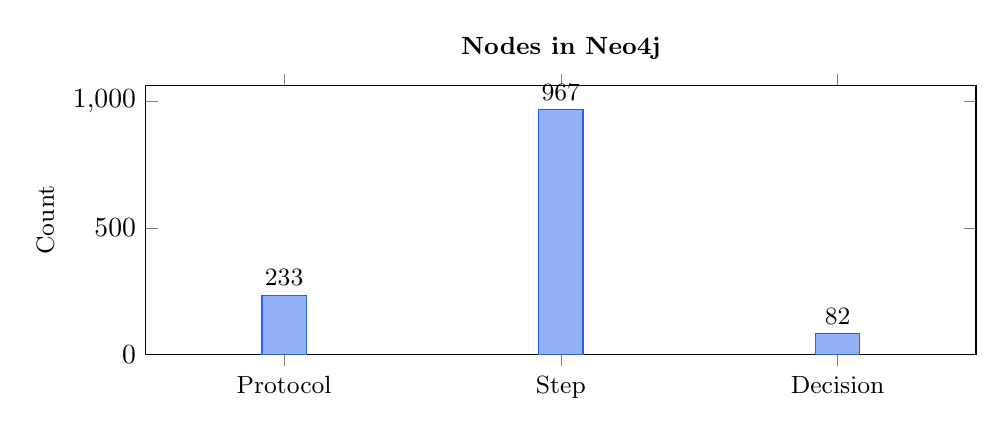
\begin{tikzpicture}
\begin{axis}[
    ybar, bar width=16pt,
    width=\textwidth, height=5cm,
    ylabel={Count}, ylabel style={font=\small},
    symbolic x coords={Protocol, Step, Decision},
    xtick=data, xticklabel style={font=\small},
    ymin=0, nodes near coords,
    every node near coord/.style={font=\small\bfseries},
    enlarge x limits=0.25,
    title={\small\bfseries Nodes in Neo4j},
]
\addplot[fill=irpgblue!50, draw=irpgblue] coordinates {
    (Protocol, 233) (Step, 967) (Decision, 82)
};
\end{axis}
\end{tikzpicture}
\end{column}
\end{columns}
\end{frame}

% ══════════════════════════════════════════════════════════════
\section{Pipeline Evolution}
% ══════════════════════════════════════════════════════════════

% ──────────────────────────────────────────────────────────────
\begin{frame}{Full F1 Timeline}
\centering
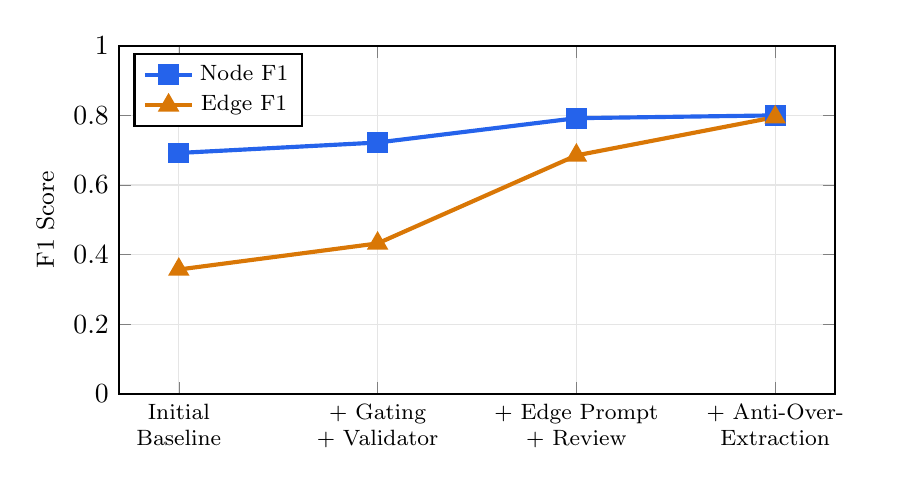
\begin{tikzpicture}
\begin{axis}[
    width=0.88\textwidth, height=6cm,
    ylabel={F1 Score}, ylabel style={font=\small},
    xtick={1,2,3,4},
    xticklabels={
        {Initial\\Baseline},
        {+ Gating\\+ Validator},
        {+ Edge Prompt\\+ Review},
        {+ Anti-Over-\\Extraction}
    },
    xticklabel style={font=\footnotesize, align=center, text width=2.5cm},
    ymin=0, ymax=1.0,
    legend style={at={(0.02,0.98)}, anchor=north west, font=\footnotesize},
    grid=major, grid style={gray!20},
    mark size=3pt, thick,
]
\addplot[color=irpgblue, mark=square*, line width=1.5pt] coordinates {
    (1, 0.692) (2, 0.722) (3, 0.792) (4, 0.800)
};
\addplot[color=vicamber, mark=triangle*, line width=1.5pt] coordinates {
    (1, 0.357) (2, 0.432) (3, 0.685) (4, 0.795)
};
\legend{Node F1, Edge F1}
\end{axis}
\end{tikzpicture}

\vspace{0.2cm}
\small Node F1: 0.692 $\rightarrow$ \textbf{0.800} (+16\%) \qquad Edge F1: 0.357 $\rightarrow$ \textbf{0.795} (+123\%)
\end{frame}

% ══════════════════════════════════════════════════════════════
\section{Next Steps}
% ══════════════════════════════════════════════════════════════

% ──────────────────────────────────────────────────────────────
\begin{frame}{Next Steps}
\begin{enumerate}
    \item \textbf{Improve edge extraction on external benchmarks}
    \begin{itemize}
        \item Chain-of-thought edge reasoning
        \item GPT-4o for edge review (instead of mini)
    \end{itemize}
    \item \textbf{Scale benchmarks}: 10 docs $\rightarrow$ full datasets (45 PET, 409 BREX)
    \item \textbf{Multilingual edge review}: fix Chinese JSON parsing
    \item \textbf{Neo4j analysis}: Cypher queries for structural patterns
    \item \textbf{Ablation study}: measure contribution of each component
    \item \textbf{Push to GitHub}
\end{enumerate}
\end{frame}

% ──────────────────────────────────────────────────────────────
\begin{frame}{Key Takeaway}
\centering
\vspace{1cm}
{\Large\bfseries Edge F1: 0.414 $\rightarrow$ 0.795 \textcolor{goldgreen}{(+92\%)}}

\vspace{0.5cm}
{\large Edge extraction bottleneck was \textbf{a prompting problem},\\not a fundamental LLM limitation.}

\vspace{0.8cm}
\begin{tabular}{lcc}
\toprule
& \textbf{Before} & \textbf{After} \\
\midrule
Node F1 & 0.679 & \textbf{0.800} \\
Edge F1 & 0.414 & \textbf{0.795} \\
Branching Accuracy & 94.4\% & \textbf{100\%} \\
External benchmark (PET Activity) & --- & \textbf{0.728} (vs.\ 0.740) \\
Neo4j protocols loaded & 0 & \textbf{233} \\
\bottomrule
\end{tabular}
\end{frame}

% ──────────────────────────────────────────────────────────────
\begin{frame}
\centering
\vspace{2cm}
{\Huge\bfseries Questions?}
\end{frame}

\end{document}
